%\documentclass{nitocs}
\documentclass[summary]{nitocs}
% \documentclass[summary,draft]{nitocs} % 画像がコンパイルされない


\usepackage[dvipdfmx]{graphicx}
\usepackage{latexsym}
\usepackage{bm}
\usepackage{amsmath}
\numberwithin{equation}{section}
\graphicspath{{./IMG/}} % 画像指定用のパス

\renewcommand{\theequation}{\arabic{equation}}
\renewcommand{\thefigure}{\arabic{section}.\arabic{figure}}
\renewcommand{\thetable}{\arabic{section}.\arabic{subsection}.\arabic{table}}
\makeatletter
\@addtoreset{equation}{section}
\@addtoreset{figure}{section}
\@addtoreset{table}{section}
\setlength{\mathindent}{0pt}
% 
\def\Underline{\setbox0\hbox\bgroup\let\\\endUnderline}
\def\endUnderline{\vphantom{y}\egroup\smash{\underline{\box0}}\\}
\def\|{\verb|}

\setcounter{page}{1}
\begin{document}

    \title{囲碁における盤面識別システムの検討}
    \author{橋本 燎}{Ryo Hashimoto} % 氏名
    \advisor{井上 優良}{Yusuke Inoue}   % 指導教員氏名

    %! 実行時の日付が自動挿入されるはず
    \date{令和3年\number\month 月\number\day 日} 

    \maketitle
    \section{緒言} \label{intro}
        囲碁は,2人のプレイヤーが碁石を碁盤へ配置するボードゲームである.碁石は各プレイヤーが使用する白黒の石であり,碁盤は通常$19\times19$の格子状の盤面のことを指す.
        %! ルール説明とかで文章を増やそう
        このゲームは両プレイヤーが碁石を交互に碁盤上に設置し,碁石で囲まれた陣地を多く確保したプレイヤーが勝利する.
        相手の陣地として成立している領域でなければどこにでも碁石を置くことができる,相手プレイヤーの碁石を陣地内に収めることでその碁石を奪い使用することで相手陣地の縮小を行うことができる等,
        ルール上の制約が極めて少ないといった特徴を持つため,他のボードゲームと比較すると可能な総局面数は膨大になる.
        % 2016年には$19\times19$の盤面における総局面数の正確な値が計算され,約$2.081681994 \times 10^{170}$通りということが明らかにされた\cite{numbers}.
        % これはオセロや将棋の総局面数を超え,観測可能な宇宙に存在する原子の総数(約$4\times10^{79}$個)よりも遥かに大きな値である.
        
        近年では,2015年にGoogle DeepMind社が開発した,ディープラーニングを実装した囲碁プログラム{\it AlphaGo}\cite{AlphaGo}が初めてプロ棋士に対しハンデ無しの対局で勝利した.
        コンピュータが人間に打ち勝つのは難しいとされていた分野で勝利を果たしたことは,人工知能の有用性を広く知らしめるものとなった.
        以降にも様々な人工知能が登場しプロ棋士との対局が行われてきたが,これらの対局の様子を見ると,プロ棋士の置いた石の配置をコンピュータに入力する役割を持った人間が存在していた.
        そこで,人の手による記録作業を行わずに対局の状況を記録できるシステムの構築を目指す.

        本研究では,対局中の囲碁の画像から碁石の配置を識別するシステムの検討を行う.
        % 段落変更対策
        具体的には,盤面を含む画像から射影変換を用いて盤面を切り抜き,ノイズ処理を適用して盤面上の線を曖昧なものにした後に,輝度値をもとに碁石の配置を識別するシステムの構築を行う.
        その後,複数の画像に対してシステムを試し,結果を考察する.

    \section{理論} \label{theory}
        \subsection{変換}
            \subsubsection{同次座標}
                座標$(x,y)$に対し,その要素を1つ増やした座標$(\xi_1,\xi_2,\xi_3)$を,以下の関係式を満たすように定義する.\\
                \begin{equation} % 同次座標の数式
                    \begin{split} % 複数行に1つの式番号を与える
                        x = \frac{\xi_1}{\xi_3} \\ 
                        y = \frac{\xi_2}{\xi_3}
                    \end{split}
                    \label{Homogeneous}
                \end{equation}

                ただし,$\xi_1,\xi_2,\xi_3$のうち少なくとも1つは0ではないとする.このように定義される座標を同次座標と呼ぶ\cite{DIP}.

                同次座標においては$\lambda\neq0$なる任意の$\lambda$に対して,$(\xi_1,\xi_2,\xi_3)$と$(\lambda\xi_1,\lambda\xi_2,\lambda\xi_3)$は通常の座標に直したときともに$(\xi_1/\xi_3,\xi_2/\xi_3)$となるため,同じ点を表している.つまり,同次座標による表現では,定数倍をしても変わらないとみなすことができる.このような表現を同値であるとよび,これを式では以下のように表す.
                \begin{equation} % 同次座標の数式2
                    \left(
                        \begin{array}{ccc}
                            \xi_1\\
                            \xi_2\\
                            \xi_3
                        \end{array}
                    \right) \sim % \sim: 「~」
                    \left(
                        \begin{array}{ccc}
                            \lambda\xi_1\\
                            \lambda\xi_2\\
                            \lambda\xi_3
                        \end{array}
                    \right)
                \end{equation}
                ここで記号$\sim$は同値関係を表し,定数倍の違いを許して等しいことを意味する.

            \subsubsection{射影変換}
                同次座標を利用することにより,一般的な変換を表現することができる.
                これは以下の式で表現されるもので,射影変換と呼ばれている\cite{DIP}.
                \begin{equation} % 射影変換の数式
                    \left(
                        \begin{array}{ccc}
                        x'\\
                        y'\\
                        1
                        \end{array}
                    \right)\sim
                    \left(
                        \begin{array}{ccc}
                        h_{11} & h_{12} & h_{13}\\
                        h_{21} & h_{22} & h_{23}\\
                        h_{31} & h_{32} & h_{33}\\
                        \end{array}
                    \right)
                    \left(
                        \begin{array}{ccc}
                        x\\
                        y\\
                        1
                        \end{array}
                    \right)
                    \label{Homography}
                \end{equation}

                射影変換においては,線分の直線性は保たれるものの,平行性は失われる.別の言い方をすると,任意の四角形を別の任意の四角形に移すような変換であるといえる.
                    %? 「概略図」? なんかパッとしない表現
                    %! 「模式図」にした
                射影変換の模式図を図\ref{sample_homography}に示す.
                \begin{figure}[tb] % 射影変換の模式図
                    \begin{center}
                    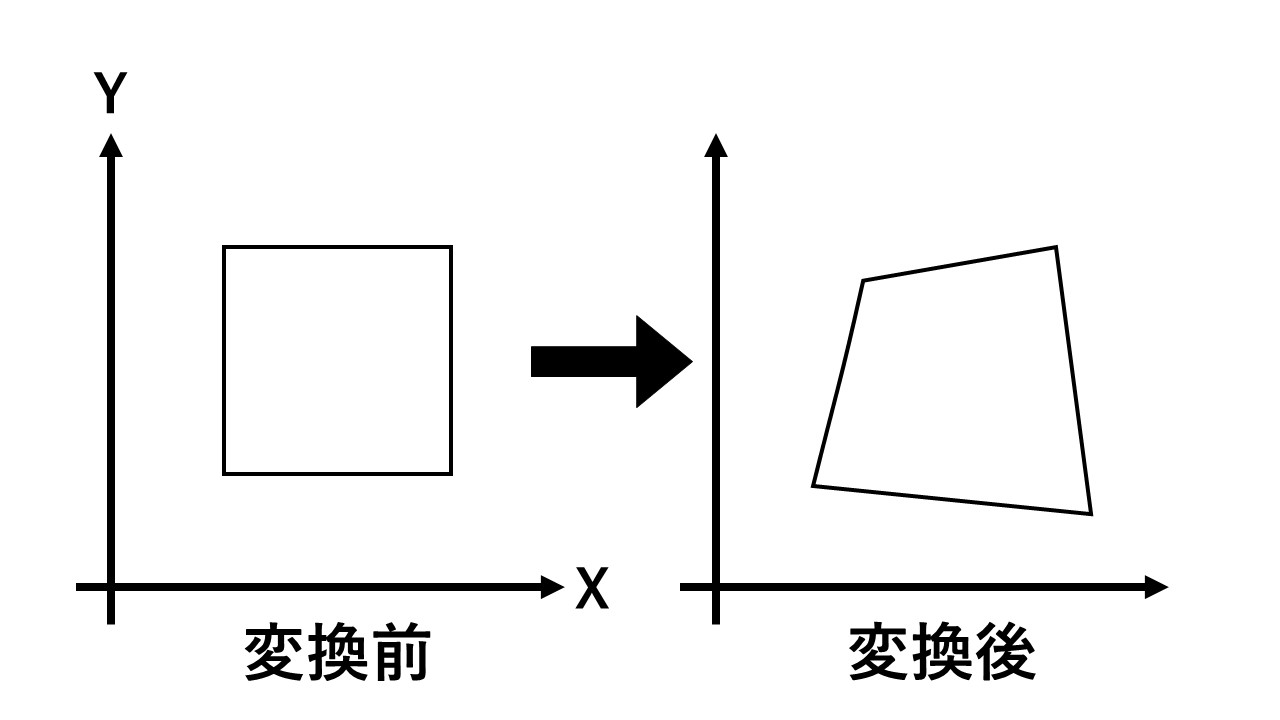
\includegraphics[clip,width=80mm]{Homography.jpg} 
                    \caption{射影変換の模式図}
                    \label{sample_homography}
                    \end{center}
                \end{figure}

    \section{システム内容} \label{system}
        システムは,与えられた画像に対して以下の前処理を行う.
        \begin{itemize}
            \item 射影変換(盤面部分の切り抜き)
            \item グレースケール化
            \item ノイズ処理
        \end{itemize}
        前処理が完了した画像に対して,システムは$19\times19$個の小さな領域を付与する.
        この領域内に存在する画素値の平均と,設定したしきい値をもとに,システムは各領域の位置に置かれている石の種類の識別を行う.
            %TODO 必要であれば領域付与済みの図を入れる

    \section{実験} \label{experiment}
        システムの有効性を検証するため,実際に盤面を含む画像を使ってシステムを適用し結果を考察する.
        %? 輝度値の決定方法について述べる余裕があるか?
        \subsection{石の位置ずれ} \label{ex2}% 位置ズレによる失敗.DSC_0099.
            この盤面画像(図\ref{ex2_img})に対し,システムを適用した.
            実際の配置と比較して,識別結果に誤りがあった部分にマークを付け,その周囲を拡大したものを図\ref{ex2_error}に示す.
            システムは図\ref{ex2_error}の誤り部分を「石がない」と識別した.

            図\ref{ex2_error}と同じ範囲の,システムによる前処理が終わって,輝度値の平均を取得する領域を緑色の四角形で表した画像を図\ref{ex2_error_area}に示す.
            図\ref{ex2_error_area}を見ると,中央の白石の大部分が領域からはみ出ているのが分かる.
            このことから,石が正しく盤面の交点上に配置されていない場合,システムは正常に石を識別できないと考える.
            
            \begin{figure}[tb] % 事例2_盤面
                \begin{center}
                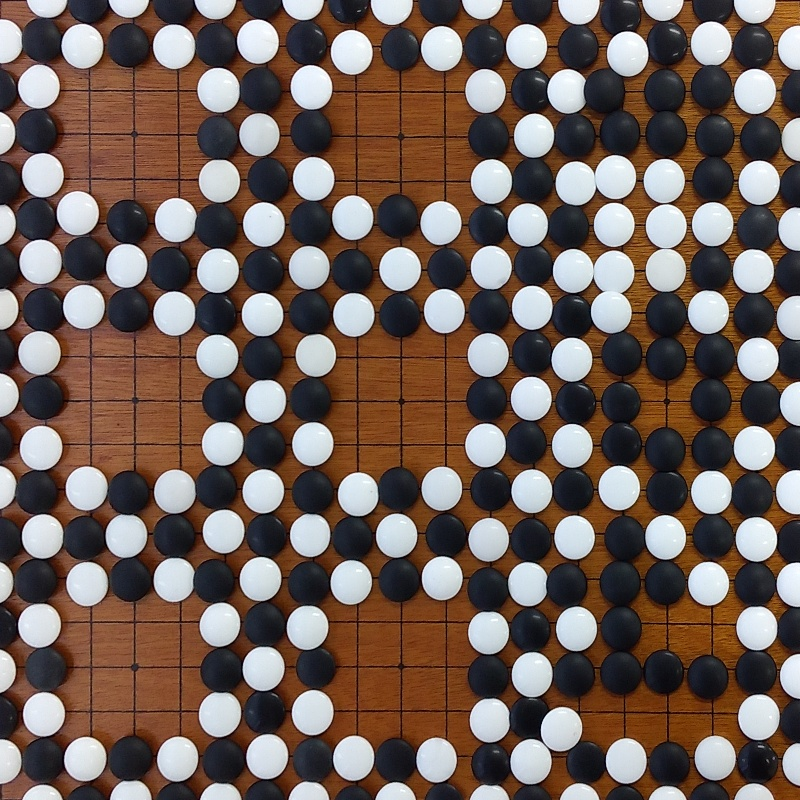
\includegraphics[clip,width=60mm]{DSC_0099/boardImg.jpg} 
                \caption{\ref{ex2}節で使用した盤面画像}
                \label{ex2_img}
                \end{center}
            \end{figure}

            %! 指摘された,誤り箇所を2枚並べにする修正
                %TODO これを論文の再提出版にも行え.
            \begin{figure}[tb] % 事例2,誤り部分・領域可視化版の2枚セット
                \begin{center}
                  \begin{tabular}{c}
                    \begin{minipage}{0.5\hsize}
                      \begin{center}
                        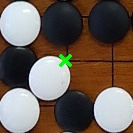
\includegraphics[clip,width=40mm]{DSC_0099/TRIM_resultCompare.jpg}
                    \caption{事例2の誤り部分}
                    \label{ex2_error}
                      \end{center}
                    \end{minipage}
                    \begin{minipage}{0.5\hsize}
                      \begin{center}
                        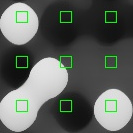
\includegraphics[clip,width=40mm]{DSC_0099/TRIM_boardWithAreaImg.jpg}
                    \caption{誤り部分の領域を可視化}
                    \label{ex2_error_area}
                      \end{center}
                    \end{minipage}
                  \end{tabular}
                \end{center}
            \end{figure}


        \subsection{碁盤の反射} \label{reflection}% 反射による失敗.DSC_0098.
            この盤面画像(図\ref{ex3})に対し,システムを適用した.
            実際の配置と比較して,識別結果に誤りがあった部分にマークを付け,その一部を拡大したものを図\ref{ex3_error}に示す.
            システムは図\ref{ex3_error}の誤り部分をすべて「白石がある」と識別した.

            図\ref{ex3_error}の範囲に対し,白石の識別に用いたしきい値よりも暗い部分を黒,明るい部分を白とした二値画像を図\ref{ex3_error_area}に示す.
            図\ref{ex3_error_area}を見ると,白石が無い部分もしきい値より明るいことが分かる.
            このことから,盤面や黒石に反射光が含まれていると,システムは誤って白石と識別してしまうと考える.
            \begin{figure}[tb] % 事例3_盤面
                \begin{center}
                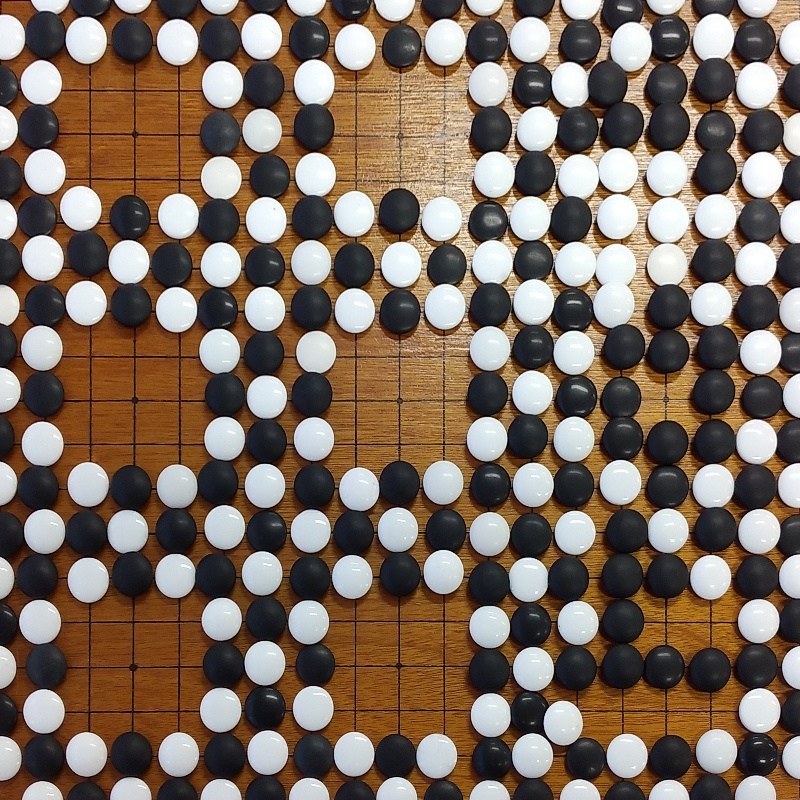
\includegraphics[clip,width=60mm]{DSC_0098/boardImg.jpg} 
                \caption{\ref{reflection}節で使用した盤面画像}
                \label{ex3}
                \end{center}
            \end{figure}

            \begin{figure}[tb] % 事例3,誤り部分,二値画像の2枚セット
                \begin{center}
                  \begin{tabular}{c}
                    \begin{minipage}{0.5\hsize}
                      \begin{center}
                        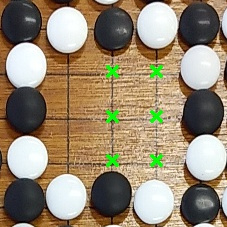
\includegraphics[clip,width=40mm]{DSC_0098/TRIM_resultCompare.jpg}
                    \caption{誤り部分の一部}
                    \label{ex3_error}
                      \end{center}
                    \end{minipage}
                    \begin{minipage}{0.5\hsize}
                      \begin{center}
                        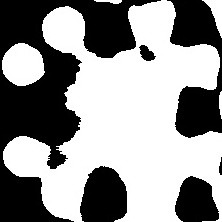
\includegraphics[clip,width=40mm]{DSC_0098/TRIM_inRange_WHITE.jpg}
                    \caption{誤り部分の二値化}
                    \label{ex3_error_area}
                      \end{center}
                    \end{minipage}
                  \end{tabular}
                \end{center}
            \end{figure}




    \section{結言}\label{conclusion} % 結言
        本研究では,囲碁の盤面を含んだ画像から碁石の配置を識別することを目的として,画像上から碁石の配置を識別するシステムの検討を行い,数件の画像に対してシステムを適用して有効性を確認した.

        \ref{experiment}章より,本研究で検討したシステムでは石の位置に大きなずれが無い,かつ反射光が写り込んでいない場合に限り,碁石を正常に識別することができた.
        石のずれに対応できない問題には,画像に付与する領域(碁石座標)の位置を等間隔ではなく,碁盤の交点や石の形状をもとに検出することでこれを解決できると考える.
        反射光を白石と識別していまう問題には,しきい値を固定するのではなく,画像の状況に応じて最適なしきい値を算出することや,画像上の反射光の写り込みを軽減させる画像処理で,誤った識別をする数を減らすことができると考える.

        したがって,今後の課題として
        \begin{itemize}
            \item 石の座標を検出する手法
            \item 画像の状況に応じて適切なしきい値を算出する手法
            \item 反射光を軽減させる画像処理の手法
        \end{itemize}
        の模索が挙げられる.    

    \begin{thebibliography}{10}
        %! 参考文献
        \bibitem{AlphaGo}
        DeepMind「AlphaGo | DeepMind」(最終閲覧日:令和3年1月13日)
        
        https://deepmind.com/research/case-studies/alphago-the-story-so-far

        \bibitem{DIP}
        ディジタル画像処理[改訂第二版],松阪 喜幸(2020)
    \end{thebibliography}

\end{document}
